\section{Discussion}
\label{section:Discussion}

\iffalse
In this section, we discuss the results of the measurements and the SEM images that were presented in the preceding chapter. Our goal during this discussion is to provide an analysis of the results that allows us to assess the quality of our devices in terms of the 

In this chapter, we analyze the results presented in the previous chapter. Our goal is to extract relevant and information regarding the quality of the fabrication as well as the quality of the devices, which we quantify by extracting several superconducting parameters from the data. Specifically, in section 5.1 we examine the fabrication results by looking at the SEM images of the devices to determine how closely the devices match the intended design. We analyse fabrication errors and the effects of the changes that were made to the design and fabrication methods. In section 5.2, we look at the temperature dependence measurements from section 4.3 of the results in order to analyse the strength of the proximity effect, which we quantify by extracting critical temperatures and the sizes of the induced energy gaps.
\fi

\subsection{Fabrication}
\subsubsection{Niobium Layer}
As can be seen in figures \ref{fig:PdNb_fabrication_SEM} and \ref{fig:AuNb_SEM}, the devices fabricated with niobium layers of 100 nm thickness are not as intended. In those images it can be seen that niobium has ended up underneath the undercut, despite being evaporated at a straight angle. In each of the imaged devices, the niobium layer covers more of the bridge than intended, and in a portion of the devices the bridge is covered completely. In the bilayer region of the device, this discrepancy between the device design and the actual device is unlikely to significantly affect the quality of the device. At the bridge, however, this fabrication error has a large effect on the quality of the device.

There are several ways in which the unintended and inconsistent placement of niobium on the bridge affects the quality of the device. First of all, if the goal is to contact a nanoscopic object with contacts made from the chosen bridge material, the contacts that are formed after the device has been electromigrated need to be made of this material. If niobium is present at or close to the electromigration site, an alloy of niobium and the bridge material may form during electromigration and the contacts that are formed will be of this alloy instead of their intended material, and the resulting device will not have the intended properties, i.e. it will have different contact resistance with the objects that it is intended to contact, and the increased scattering caused by the mixture of materials will reduce superconductivity since the Thouless energy scales with the square root of the diffusion coefficient. 

Secondly, the inconsistency of the placement of niobium on the bridge means that experiments done using these devices will be less reproducible and the experimental conditions will be less controlled.


The presence of niobium in the undercut was hypothesized to be due to film stress in the niobium. The solution that was tried was to reduce the thickness of the niobium layer to 50 nm and to increase the rate of evaporation to 0.5 nm/s. As can be seen in figures \ref{fig:AuNbV3_SEM} and \ref{fig:AuNb60nm_SEM}, the devices that were made with these niobium evaporation parameters have niobium layers that closely match the shape of the patterned design, without the clear presence of niobium in the undercut, including on the bridge. The conclusion drawn from these images is that evaporating the niobium with the new parameters has resolved the issue that was present in the preceding devices. 

\iffalse
Based on the SEM images of the devices, we see that the distance between the corners of the niobium layers on opposite sides of the bridge is between 50 and 60 nm in the AuNb devices with 50 nm niobium thickness, which is in accordance with the distance of 50 nm specified in the design. In the AuNb devices with 60 nm bridge spacing, however, the shortest distance between the niobium layers is between 90 nm and 100 nm, which deviates from the design by over half the distance specified in the design pattern. A possible explanation for this deviation is that the e-beam exposure dose was not changed when the design pattern was changed from 50 nm to 60 nm. Since the regions close to the edge of the pattern on either side of the bridge recieve fewer secondary electrons from the other side of the bridge when the spacing is increased, the effective dose is reduced. If the goal is to match the distance in the design, therefore, the exposure dose needs to be increased when the patterned bridge distance is increased. However, we selected this pattern becuase on SEM images of a spacing test. In the spacing test, this was the design that minimized the overlap between the gold layers at the center of the bridge. Based on our test, the overlap was minimized wen the bridge spacing as 90 nm, which we achieved by patterning 60 nm and using the same dose as in the prior designs. The discrepancy between the patterned design and the resulting device is not problematic as long as we are aware that whenever we refer to the AuNb device with 60 nm bridge spacing, we are talking about a device with a bridge that is 90 nm in length.
\fi

\subsubsection{Bridge}
The images in figure \ref{fig:AuNbV3_SEM} show a region of higher brightness in the center of the bridge. We also see based on the rest of the image that this is the region at which the two gold layers that were evaporated at different angles overlap. Based on this reasoning, we can associate the region of increased brightness with a gold layer that is twice as thick as intended. 

The reason that a bowtie geometry is used is that electromigration is most likely to start in regions of higher local resistivity and current density. The bowtie geometry is designed to create a single point of maximal resistivity and current density at the center of the bridge, in order to make electromigration consistent and reproducible between different devices, and to ensure that the resulting device has optimal superconducting properties.

When the gold layers overlap in the center and double the local gold thickness there, this reduces the local current density and resistivity in that region. This makes electromigration less likely to take place in the center, and more likely to take place asymmetrically, near either end of the bridge.\\


In order to eliminate the region of overlap between the gold layers, the bridge spacing was increased from 50 nm to 60 nm. As can be seen in figure \ref{fig:AuNb60nm_SEM}, the devices that were made with this bridge spacing do not show a clear region of overlap. Another consequence of the new spacing is that the center of the geometry is more constricted than before. Both these changes ensure that the local resistivity and current density is maximal in the center of the bridge. 

The plot in figure \ref{fig:Migration_stats} shows that the there is less spread in the resistance values of the devices with 60 nm spacing after migration, which indicates a higher degree of control during the electromigration process. However, since the electromigration in the 60 nm devices was done cold and the electromigration in the 50 nm devices at room temperature, it is difficult to separate the effect of these two changes and it is not possible to draw strong conclusions from this data. When looking at the electromigration curves in appendix E3 and E4, we see that the critical voltage required to start the migration process is lower on average for the devices with 60 nm bridge spacing, and that the steps in the resistance of the device are smaller on average in those devices as well. Both of these differences indicate that electromigration is more controllable in the devices with 60 nm bridge spacing. 


\subsection{Transport Measurements Before Electromigration}

Since our goal is to characterize our SEMBJ devices, there are several parameters that we are interested in which quantify the superconductivity. Two of the most important parameters are the Thouless energy and the energy gap of the bilayer.

%including the electronic diffusion coefficient in the bridge, $D$, the Thouless energy $E_{Th}$, the superconducting coherence lengths in the superconductor and in the normal metal, and the superconducting energy gap in the bulk film. 

Determining these parameters in the device before electromigration can help characterize the electromigrated device, as well as the way the properties of the device are changed during the electromigration process. Since electromigration is expected to only change the structure of the device in the bridge while leaving the bulk film unaltered, we can reasonably assume that the bulk film properties, including $|\Delta|$, are not significantly altered by electromigration. Although we can not say the same thing about the Thouless energy, knowing what the value of the Thouless energy was before migration took place may give insight into the way electromigration changes the structure of the bridge.

%diffusion constant in the bridge, the thouless energy of the device and $\xi_N$, it is still valuable to know what these values were 





%The hypothesis is that the transport measurements in the devices before electromigration are useful for determining these values. Since electromigration is expect to only change the structure of the device in the bridge while leaving the bulk film unaltered, we can reasonably assume that the bulk film properties $\Delta$ and $\xi_S$ are not significantly altered by electromigration. Although we can not say the same thing about the diffusion constant in the bridge, the thouless energy of the device and $\xi_N$, it is still valuable to know what these values were before migration took place. Knowing this might give insight into the way electromigration changes the structure of the bridge. Although electromigration changes the shape of the bridge and its grain structure, which will change $D$, $E_{Th}$ and $\xi_N$, it seems unlikely that the changes will be on the order of several orders of magnitude. Therefore, the values of these quantities can also be used as rough estimates for the values after electromigration.


\subsubsection*{Device Properties Before Electromigration}

The critical voltage, $V_C = I_CR_N$, is an important quantity that quantifies the transport properties of the devices. The values of the critical current and normal state bridge resistance have been extracted from the VI measurements of the devices, as is discussed in the results. For each type of device, the $I_CR_N$ product has been calculated for each device and has been plotted as a function of $R_N$ in figure \ref{fig:IcRn_Products}. In order to quantify the degree to which the fabricated devices vary, we calculate the coefficient of variation of the $I_CR_N$ products for each device type. We also calculate the correlation coefficient between $I_CR_N$ and $R_N$. The values we get are shown in table \ref{tab:IcRn_Products}.

\begin{figure}[H]
     \centering
     \begin{subfigure}[b]{0.49\textwidth}
         \centering
         \includegraphics[width=\textwidth]{/Discussion/IcRn_PdNb.png}
         \caption{PdNb.}
         \vspace{5mm}
         %\label{a}
     \end{subfigure}
     \hfill
     \begin{subfigure}[b]{0.49\textwidth}
         \centering
         \includegraphics[width=\textwidth]{/Discussion/IcRn_AuNbV2.png}
         \caption{AuNb.}
         \vspace{5mm}
         %\label{b}
     \end{subfigure}
     \hfill
     \begin{subfigure}[b]{0.49\textwidth}
         \centering
         \includegraphics[width=\textwidth]{/Discussion/IcRn_AuNb, 50nm Nb.png}
         \caption{AuNb with 50 nm niobium.}
         %\label{c}
     \end{subfigure}
     \hfill
     \begin{subfigure}[b]{0.49\textwidth}
         \centering
         \includegraphics[width=\textwidth]{/Discussion/IcRn_AuNb, 60 nm Spacing.png}
         \caption{AuNb with 60 nm bridge spacing.}
         %\label{d}
     \end{subfigure}
        \caption{Scatter plots of the $I_CR_N$ products of the devices, as a function of $R_N$.}
        \label{fig:IcRn_Products}
        
\end{figure}

\begin{table}[H]
\caption{Coefficient of variation, defined as the ratio between the standard deviation and the mean, of the $I_CR_N$ products of the different types of devices, as well as the correlation coefficient between the $I_CR_N$ products and the normal state bridge resistances of the devices.}
\label{tab:IcRn_Products}
\begin{tabular}{|c|c|c|}
\hline 
Device & Coefficient of Variation & Correlation Coefficient \\ 
\hline 
PdNb & 65.9\% & 0.003 \\ 
\hline 
AuNb & 13.8\% & 0.99 \\ 
\hline 
AuNb, 50 nm Nb & 7.2\% & -0.64 \\ 
\hline 
AuNb, 90 nm Spacing & 27.6\% & -0.80 \\ 
\hline 
\end{tabular} 

\end{table}

The reason that we are interested in $I_CR_N$ as a function of $R_N$, is that, with minimal changes to the device design, $R_N$ could be measured at room temperature using a 4 point measurement. If there is a correlation between $I_CR_N$ and $R_N$, the $R_N$ value can then be used to select the junctions that are likely to have a high $I_CR_N$ product based on this correlation. If there is no correlation or only a very weak correlation, the junctions with the highest $R_N$ value can be chosen, since a higher value of $R_N$ improves electromigration.  The PdNb devices show the most variation in their $I_CR_N$ product. Based on the SEM images of these devices, we know that their fabrication was very inconsistent, so this is not a surprising result. The correlation coefficients don't show a pattern across devices. The $I_CR_N$ product of the PdNb device is not correlated to its normal state bridge resistance. The other devices show strong correlations, but not in a consistent direction. Further research would be needed to determine the underlying causes of these differences. Doing so would be worthwhile, especially if it would allow us to intentionally create a strong positive correlation, such as the AuNb devices show here. If that were possible, those devices could be selected based on simple room temperature measurements that have a high normal state bridge resistance as well as a high expected $I_CR_N$ product. Although we were not able to determine the mechanism which determines the correlation between $I_CR_N$ and $R_N$, this discussion does show that if the correlation coefficient of a set of devices is known, it can be usefully employed in device selection before the devices are loaded into a measurement setup and cooled. 

\subsubsection{Critical Temperature}

In the VIT measurements of the devices, such as for example figure \ref{fig:AuNbV2_VIT}, we can distinguish three distinct regions. In the region of low temperature and low current, the resistance of the device is lowest. We interpret this as the region in which the both the bridge and the bulk film are superconducting. Because the bridge has a smaller cross-section than the bulk film, the local current density is higher there than in the bulk film. Therefore, the critical current density is reached at a lower total current. Furthermore, in the devices where there is no niobium on the bridge, the bridge material is proximitized less strongly than it is in the bulk film, since the degree of proximitization decreases as the distance to the superconductor increases. Therefore, in the bridge, the critical temperature and current density are lower than in the bulk film. The critical current of the bridge can be seen in the VIT measurements as a function of temperature, as two converging lines of high differential resistance separating the region of lowest device resistance from a region of higher device resistance. The critical current in these plots decreases as a function of temperature, as expected. In this region of higher device resistance the bridge is no longer superconducting, but the bulk film still is. At higher temperature, there is a sharp transition as the temperature exceeds the critical temperature of the bulk film, and the entire device transitions to the normal state. Since the cross section of the bulk film is much larger than that of the bridge, the current range of the measurement is too small to resolve the critical current of the bulk film as a function of temperature. 

We can extract the differential resistance of the device at zero bias current from the VIT measurements. In such a plot, we can identify three regions of relatively constant resistance, separated by regions of large gradient of resistance as a function of temperature. The critical temperature is taken to be the temperature at which the resistance is halfway between the normal state resistance and the superconducting state resistance. An example of such an extraction is shown in figure \ref{fig:TC_extraction}.

\begin{figure}[H]
     %These plots come from numid 2 from PdNb chip 6
     \centering
     \begin{subfigure}[t]{0.66\textwidth}
         \centering
         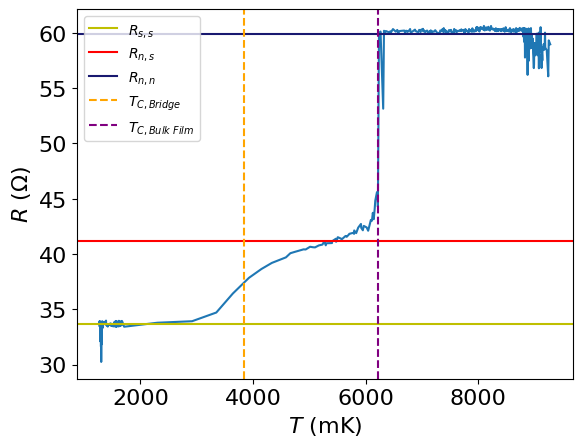
\includegraphics[width=\textwidth]{Discussion/PdNb_Rt_Tc_extraction.png}
         %\caption{Representative VIT}
         \label{subfig:}
     \end{subfigure}
     \caption{Representative graph showing the zero bias current differential resistance as a function of temperature. }
     \label{fig:TC_extraction}
        
\end{figure}

We also extract the width of the superconducting transition, $\Delta T_C = T90\% - T10\% $, where $T90\% $ and $T10\% $ are the temperatures corresponding to $90\% $ and $10\% $ of the resistivity jumps, respectively. All the extracted critical temperatures and their widths for the different devices are shown in table \ref{tab:TC_extraction}.



In order to establish a relationship between the critical temperature in the bulk film and the critical temperature in the bridge, we also show the ratio of these two temperatures in table \ref{tab:TC_extraction}. 

\begin{table}[H]
\caption{$T_C$ and $\Delta T_C$ values for the bridge and bulk film in the different devices, in mK, as well as the ratios of the bridge $T_C$ and bulk film $T_C$, the ratio of the bulk film $T_C$ and the $T_C$ of a bare niobium layer of the same thickness, and transparency as fitted using eq. \ref{eq:BilayerTc} from the theory. Bridge $T_C$ not clearly defined for the AuNb device with 50 nm Nb and 50 nm spacing.}
\label{tab:TC_extraction}
\centering
\begin{tabular}{|c|c|c|c|c|c|c|c|}
\hline 
Device & $T_{C, B}$ & $\Delta T_{C, B}$ & $T_{C, BF}$  & $\Delta T_{C, BF}$ \\ 
\hline 
PdNb & 3844 & 1669 & 6226 & 112 \\ 
\hline 
\makecell{AuNb, \\ 100 nm Nb} & 5132 & 1303 & 8853 & 1086 \\ 
\hline 
\makecell{AuNb, 50 nm Nb, \\ 50 nm Spacing} & $\approx$ 5800 & - & 8804 & 899 \\ 
\hline 
\end{tabular} 

\end{table}

Using the obtained $T_C$ value for the bulk film, we can immediately calculate the superconducting energy gap of the bulk film using the equality $\Delta = 1.764k_BT_C$. The energy gaps thus obtained  are tabulated in table \ref{tab:TC_extraction_calculations}. 


As mentioned in the chapter on theory, pure niobium films of 50 nm and 100 nm thickness have respective critical temperatures of 8.9 K and 9.1 K approximately. If we compare the bulk film critical temperatures in table \ref{tab:TC_extraction} to these values, can give us a measure of the degree to which the bilayers are (inversely) proximitized. The ratio between the bulk film critical temperature and the critical temperature of a pure niobium layer with corresponding thickness, is shown in table \ref{tab:TC_extraction_calculations}.

\iffalse
\noindent \textbf{Interface Transparency Fit}
The devices studied in this thesis can be modelled as SN-bilayer normal metal SN-bilayer junctions. The bulk film $T_C$ is the $T_C$ of the SN-bilayer. In equation \ref{eq:BilayerTc} on the critical temperature of an SN bilayer, for each device type all parameters are known except for the interface transparency $t$. This means that we can use equation \ref{eq:BilayerTc} to fit the interface transparency. One detail is of note in this procedure, namely that the films are not truely bilayers, but in fact trilayers since there is a 5 nm Ti sticking layer in each case. Looking at table \ref{tab:Bilayer_Table}, we see that the density of states at the Fermi energy is of the same order for Au and Ti, while the density of states at the Fermi energy of Pd is an order of magnitude larger. Based on this, we hypothesise that the Ti layer has negligable influence on the critical temperature in Pd-bridged devices, and we omit it in the fit. In the case of Au-brided devices, we cannot assume that the influence of the Ti layer is negligible, since Ti has a density of states at the Fermi energy that is larger than that of Au. The influence of the Ti layer on the bulk film critical temperature is reduced, however, if the interface transparency is less than one. Because the Ti layer and Au layer are evaporated in the same evaporator, and the device is kept under high vacuum in between the evaporation of the two layers, we assume that the interface transparency is less than but on the order of one. The effect Ti has on lowering the $T_C$ is also mitigated to some degree by the fact that Ti has a critical temperature that is slightly higher than zero (is that true? not sure). Based on these condsideraions, we then make the simplifying approximation that we can use the density of states at the Fermi energy for gold for the value of $n_n$ in equation \ref{eq:BilayerTc}, and simply add the thicknesses of the Ti and Au layer to arrive at $d_n$. The values found by fitting the transparency coefficient $t$ in this way are also shown in table \ref{tab:TC_extraction_calculations}.\\
\fi

\begin{table}[H]
\caption{The ratio of the bulk film $T_C$ and the $T_C$ of a bare niobium layer of the same thickness,$\frac{T_{C, B}}{T_{C,Nb}}$ as well as the ratio of the critical temperatures of the bridge and the bulk film, $\frac{T_{C, B}}{T_{C,Nb}}$ and the bilayer energy gap $\Delta_{BF}$.}
\label{tab:TC_extraction_calculations}
\centering
\begin{tabular}{|c|c|c|c|c|c|c|c|}
\hline 
Device &  $\frac{T_{C, B}}{T_{C,Nb}}$ & $\frac{T_{C, B}}{T_{C,BF}}$  & $\Delta_{BF}$\\ 
\hline 
PdNb & 67\% & 62\%  & 0.95 meV\\ 
\hline 
\makecell{AuNb, \\ 100 nm Nb} &  99.4\% & 58\%  & 1.35 meV\\ 
\hline 
\makecell{AuNb, 50 nm Nb, \\ 50 nm Spacing} & 98.9\% & 66\%  & 1.34 meV\\ 
\hline 
\end{tabular} 

\end{table}


For the AuNb devices with 60 nm bridge spacing, no VIT measurement was done. Since only the bridge design was changed, and the bulk film fabrication was identical to the AuNb devices with 50 nm niobium and 50 nm bridge spacing, we can assume that the bulk film properties of these two device types are similar. Since the bridge dimensions are changed between the two device designs, a similar extrapolation for the bridge $T_C$ is difficult, but based on the theory it seems reasonable to assume that the bridge $T_C$ is on average lower in the 60 nm bridge spacing devices, since the strength of the proximity effect decreases with distance.


In table \ref{tab:TC_extraction} we see that for all devices the ratios between the critical temperature of the bridge and the critical temperature of the bulk film are all within a few percent of 60\%. This suggests that there is a consistent relationship between the critical temperature of the bulk film and that of the bridge, and that the critical temperature of the bulk film is therefore a relevant quantity when investigating the critical temperature of the bridge. 

%\noindent \textbf{Agreement with Theory}\\
Based on table \ref{tab:TC_extraction}, we can conclude that changing the bridge material from palladium to gold led to a higher critical temperature for the device. This agrees with our expectations based on equation \ref{eq:BilayerTc}, since gold has a much lower density of states at the Fermi energy compared to niobium. 

%In fact, if we use equation \ref{eq:BilayerTc} to calculate the ratio between the critical temperatures of the two devices, assuming a transparency of 0.5 for both, we find that this ratio is 0.697. The ratio of bulk film critical temperatures in table \ref{tab:TC_extraction} is 0.712, which is in good quantative agreement with this prediction, despite the fact that the transparency as given by the fit is not constant.

Table \ref{tab:TC_extraction} also shows that the changes that were made as the device design was iterated from the AuNb design with 100 nm Nb to the AuNb design with 50 nm Nb made only a small difference in terms of the critical temperature of the bulk film.

% The graph of $T_C$ as a function of Nb thickness predicted by equation \ref{eq:BilayerTc}, using the parameters corresponding to the AuNb device with 100 nm Nb and a transparency of 0.15, is plotted in figure \ref{fig:palladium_thickness_tc_theory}. In this plot we see that at 100 nm Nb thickness the theory predicts that we are already far in the asymptotic regime, where the partial derivative of the bilayer critical temperature with respect to the thickness of the superconductor is relatively small. Quantitatively, equation \ref{eq:BilayerTc} predicts that the critical temperature is reduced by only 0.15\% when the thickness of the gold layer is increased from 26 nm to 30 nm and the thickness of the niobium is reduced from 100 nm to 50 nm, assuming that the transparency coefficient remains at 0.15.

\iffalse
\begin{figure}[H]
     %These plots come from numid 2 from PdNb chip 6
     \centering
     \begin{subfigure}[t]{0.66\textwidth}
         \centering
         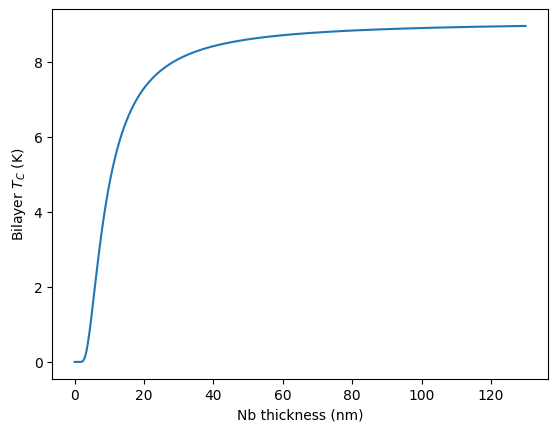
\includegraphics[width=\textwidth]{Bilayer_Tc_Theory_Graph.png}
         %\caption{Representative VIT}
         \label{subfig:}
     \end{subfigure}
     \caption{Graph showing the predicted $T_C$ value of a gold-niobium bilayer as a function of the thickness of the niobium layer. The graph assumes a transparency of 0.15 and a gold layer thickness of 26 nm. Graph based on equation \ref{eq:BilayerTc}.}
     \label{fig:palladium_thickness_tc_theory}
        
\end{figure}

\fi


%The transparency values that were fitted are shown in table \ref{tab:TC_extraction}. One thing that stands out in these data is that the interface transparency of the PdNb device is much higher than the interface transparency of both AuNb devices. A factor that likely contributes to this difference is the fact that 

The interface transparency between the bridge material and niobium layer is an important parameter that determines how well the superconducting electrons are able to enter the bridge and thereby induce superconductivity. The fact that we see induced energy gaps of the order of the energy gap of bare niobium implies that the interface transparency is sufficiently high. One aspect of fabrication that may have a particularly strong influence on the interface transparency is the exposure of the normal metal film before the evaporation of the niobium layer. Palladium and niobium are evaporated in the same evaporator, while gold and niobium are evaporated in different evaporators. This means that in the case of gold-bridged devices, the gold surface is exposed to air during the transport between the two evaporators, which may allow for contaminants to reduce the pristineness of the gold-niobium interface. The PdNb devices, on the other hand, remain in high vacuum between the evaporation of palladium and niobium and thereby minimize the amount of contamination at the interface. Since the interface transparency is an important parameter governing the quality of the superconductivity in the bridge, steps should be taken to ensure that its value is maximized. Ideally, an evaporator would be used in which both gold and niobium are available. In case that is not possible, the time in which the device is exposed to air in between the evaporation of gold and niobium should be minimized. \\

  






\iffalse
\subsubsection*{Bridge Resistance}

When looking at the IV meaurements that were done on the devices before breaking it stands out that all the devices have a near consant differential resistance around zero bias current, which then makes a sharp transition and ends up at a near constant higher resistance. As mentioned, we can interpret this as a sign of superconductivity, and associate the current of the jump with the critical current of the bridge. All the measured devices show this behavior, and so we can conclude that all the devices are superconducting before breaking. We also note that the ability to extract the normal state bridge resistance from a VI measurement is something that would be impossible in a device that does not incorporate superconductivity, which is one of the benefits SEMBJs have over normal state EMBJs. 

In order to estimate the effective length of the bridge, and to validate the normal state bridge resistances in our results, we estimate the normal state bridge resistance of the AuNb device with 50 nm niobium using a SEM image of the device before breaking and the literature values for the resistivity of thin gold films. 

Looking at the SEM image of the AuNb device with 50 nm niobium, we estimate the bridge to be the region of gold film in between the corners of the niobium layer. This region is next approximated with three rectangles, as is shown in figure \ref{fig:BridgeResistanceExtraction}. Based on the discussion on the fabrication results, we know that the thickness of the gold film in the yellow regions is 15 nm, while in the orange region it is 30 nm. We can estimate the height and width of the rectangles using the scale bar of the SEM image. Using the literature values of the resistivity of 15 nm and 30 nm thick gold films (191 $\Omega$nm and 40 $\Omega$nm respectively), we can then calculate the total resistance of the three rectangles, which we model as three resistances in series. The result of this calculation is a resistance of 6.1 $\Omega$. As can be seen in figure \ref{fig:AuNbV3_VI}, the values for the normal state bridge resistance that were extracted from the measurements for these devices are all in the range of 5 to 6 $\Omega$. Therefore we can conclude that the effective length of the junction is close to its geometric length of 50 nm, and that the results of the VI measurements, and our interpretation of those results, are reasonable.


\begin{figure}[H]
     %These plots come from numid 2 from PdNb chip 6
     \centering
     \begin{subfigure}[t]{0.66\textwidth}
         \centering
         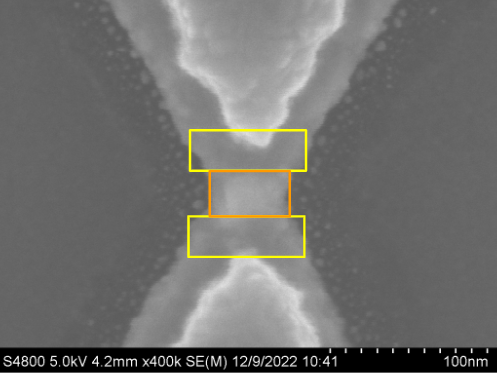
\includegraphics[width=\textwidth]{BridgeREstimate.png}
         %\caption{Representative VIT}
         \label{subfig:}
     \end{subfigure}
     \caption{Graph showing the predicted $T_C$ value of a gold-niobium bilayer as a function of the thickness of the niobium layer. The graph assumes a transparency of 0.15 and a gold layer thickness of 26 nm. Graph based on equation \ref{eq:BilayerTc}.}
     \label{fig:BridgeResistanceExtraction}
        
\end{figure}
\fi


 




\subsubsection{Thouless Energy}

Using equations \ref{eq:E_Th(D,L)} and \ref{eq:Xi_N_of_T}, we can express the Thouless energy purely as a function of the ratio $L/\xi_N(T_C)$ and $T_C$: 

$$E_{Th}\left(\frac{L}{\xi_N(T_C)}\right) = 2\pi k_BT_C / \left(\frac{L}{\xi_N(T_C)}\right)^2$$

Since $T_C$ is known for the devices, we can get the ratio $L/\xi_N(T_C)$ from figure \ref{fig:V_C_of_T_for_different_L_over_Xi} and the critical voltage of the devices as a function of temperature. 


In order to determine $V_C(T)$, we need $I_C(T)$ and $R_N$. The critical current can be extracted as a function of temperature from a VIT measurement simply by taking the argmax of the differential resistance as a function of current at each temperature. The result of such an extraction is plotted in figure \ref{fig:IcExtraction} for the IVT plot from figure \ref{fig:AuNbV2_VIT} from the results. 

\begin{figure}[H]
     %These plots come from numid 2 from PdNb chip 6
     \centering
     \begin{subfigure}[t]{0.66\textwidth}
         \centering
         \includegraphics[width=\textwidth]{/Discussion/IcExtraction.png}
         %\caption{Representative VIT}
         \label{subfig:}
     \end{subfigure}
     \caption{Illustration of the extraction of $I_C$ as a function of temperature from a VIT measurement.}
     \label{fig:IcExtraction}
        
\end{figure}

Since $R_N$ has been determined for each device, we can obtain $V_C = I_CR_N(T)$ by multiplying $I_C(T)$ with $R_N$. We can then rescale the temperature and $V_C$ in the same way as they are scaled in figure \ref{fig:V_C_of_T_for_different_L_over_Xi}, such that we can compare our devices with that plot. The extracted values of $I_CR_N$ have been plotted for each device for which a VIT measurement was done, and the lines from figure \ref{fig:V_C_of_T_for_different_L_over_Xi} have been reproduced in order to facilitate comparison. The result is shown in figure \ref{fig:likharev_plot}. We can use this plot to extract the ratio $\xi_N(T_C) / L$. We can also gauge the degree to which our measurements are described by the theory, by how well the temperature dependence of the $I_CR_N$ products follows the shapes of the curves in figure \ref{fig:V_C_of_T_for_different_L_over_Xi}. We see that the curves closely follow the shape of the curves from the theory, indicating the validity. In the case of the AuNb devices with 60 nm bridge spacing, no VIT measurement was done, and for this device the average of all $I_CR_N$ values, which were all obtained at the same temperature, is used. 

\begin{figure}[H]
     %These plots come from numid 2 from PdNb chip 6
     \centering
     \begin{subfigure}[t]{0.66\textwidth}
         \centering
         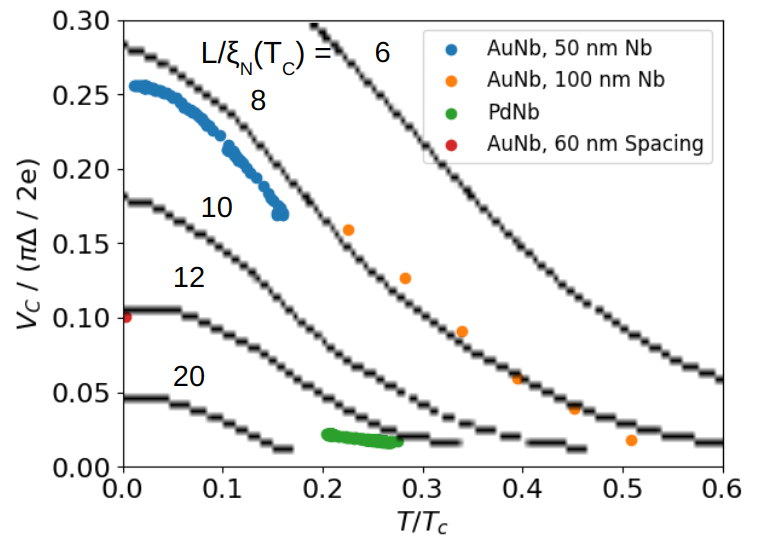
\includegraphics[width=\textwidth]{Likharev_plot_all4.png}
         %\caption{Representative VIT}
         \label{subfig:}
     \end{subfigure}
     \caption{Comparison of $I_CR_N(T)$ with the theoretical result extracted from figure \ref{fig:V_C_of_T_for_different_L_over_Xi}.}
     \label{fig:likharev_plot}
        
\end{figure}

From this figure, we can estimate the ratio $L/\xi_N$ to be approximately 8 for the AuNb device, 12 for the average AuNb device with 60 nm spacing, 8.5 for the AuNb device with 50 nm niobium, and somewhere between 12 and 20 for the PdNb devices. For the PdNb device the estimation is more difficult, but we will choose 14 for our estimate. Finally, we find the Thouless energies by substituting these values into the equation above. The obtained values are shown in table \ref{tab:E_Th_SNS}.

\begin{table}[H]
\caption{Thouless energy calculated using the $L/\xi_N(T_C)$ value obtained above for each device type.}
\label{tab:E_Th_SNS}
\centering
\begin{tabular}{|c|c|c|c|c|c|}
\hline 
Device &  $E_{Th}$ ($\mu$eV)\\ 
\hline 
PdNb & 18  \\ 
\hline 
AuNb &  75 \\ 
\hline 
AuNb, 50 nm Nb & 67  \\ 
\hline 
AuNb, 60 nm Spacing & 33   \\ 
\hline 
\end{tabular} 

\end{table}

\iffalse
\subsection*{$\xi_N, D, l$ and $L$}

The devices can be further characterized by determining the superconducting coherence length, diffusion coefficient, mean free path and effective device length. Since we know the thouless energies of the devices, we only require one of these parameters to determine all the others, using formulas \ref{eq:E_Th(D,L)}, \ref{eq:Xi_N_of_T} and $D = v_f*l/3$. We will estimate the mean free path using the literature values of the film resistances corresponding to our bridge materials. Since the bridges are constricted films and not bulk films, this estimate is likely to overestimate the actual mean free path length, since the constriction in the film causes additional surface scattering. We use the following relationships between the resistivity and mean free path of palladium and gold: for palladium $rho*l = $
\fi

\iffalse
Using the relationship $l*\rho$ = 835 $\Omega$nm$^2$ \cite{Electron mean free path in elemental metals} and the resistivities of 13 nm and 15 nm thick gold layers (2.28 $\Omega\mu$m and 190 $\Omega$nm, respectively \cite{Electrical resistivity of gold thin film as a function of film
thickness}) we can obtain a rough estimate of $l$ in the gold bridged devices. Since the gold layers are constricted, the added boundary scattering caused by the constriction relative to a bulk film means that we expect this estimate of $l$ to be too high. 

\begin{table}[H]
\caption{}
\label{tab:likharev_table}
\centering
\begin{tabular}{|c|c|c|c|c|c|}
\hline 
Device & $L$ (nm) & $\xi_N(T_C)$ (nm) & $D$ (cm$^2$/s) & $E_{Th}$ ($\mu$eV) & $l$ (nm) \\ 
\hline 
PdNb & & 3.6 & 0.66 & 17.5 & 0.20 \\ 
\hline 
AuNb & 38.4 & 4.8 & 1.7 & 75.2 & 0.37 \\ 
\hline 
AuNb, 50 nm Nb & 141 & 16.7 & 20.1 & 66.7 & 4.37 \\ 

\hline 
\end{tabular} 

\end{table}

----------------\\
We know that for the AuNb devices with 50 nm niobium, the gap sizes are consistently close to 50 nm. For the PdNb devices and the AuNb devices with 100 nm niobium, however, we know that the bridge length is often lower than intended in the design. We will still take $L$ to be 50 nm in those devices, and keep in mind that this is an imprecise estimate for these devices.

Looking at figure \ref{fig:likharev_plot}, we see that the shape of the $I_CR_N$ curves of our devices match the shapes of the theoretical figure. The AuNb device with 50 nm niobium matches the shape most closely, and for the PdNb device the degree of agreement is most difficult to estimate, due to the small temperature range and low value of its critical voltage.

From this figure, we can estimate the ratio $L/\xi_N$ to be approximately 8 for the AuNb device, 8.5 for the AuNb device with 50 nm niobium, and somewhere between 12 and 20 for the PdNb devices. For the PdNb devise the estimation is more difficult, but we will choose 14 for our estimate. These ratio's allow us to calculate $\xi_N(T_C)$. The values obtained for $\xi_N(T_C)$ in this way are 5.9 nm for the AuNb device with 50 nm niobium, 6.3 nm for the AuNb device with 100 nm niobium, and 3.6 for the PdNb device. These values have been tabbulated in table \ref{tab:likharev_table}.

Usign equation \ref{eq:Xi_N_of_T}, we can then find the value of $D$, the normal metal diffusion constant. In turn, we can use $E_{Th} = D\hbar/L^2$ and $D = v_Fl/3$ to calculate the Thouless energy and electron mean free path in the bridge. All the calculated values are shown in table \ref{tab:likharev_table}.

-----------------

\begin{table}[H]
\caption{}
\label{tab:likharev_table}
\centering
\begin{tabular}{|c|c|c|c|c|}
\hline 
Device & $\xi_N(T_C)$ (nm) & $D$ (cm$^2$/s) & $E_{Th}$ ($\mu$eV) & $l$ (nm) \\ 
\hline 
PdNb & 3.6 & 0.66 & 17.5 & 0.20 \\ 
\hline 
AuNb & 6.3 & 2.89 & 76.1 & 0.62 \\ 
\hline 
AuNb, 50 nm Nb & 5.9 & 2.52 & 66.3 & 0.54 \\ 
\hline 
AuNb, 60 nm Spacing & 3.8 & 1.04 & 19.0 $\pm$ 4.9 & 0.31 \\ 
\hline 
\end{tabular} 

\end{table}

Discussion of the table.


\noindent A second method for calculating these quantities is using formulas \ref{eq:IcRn_at_low_T} and \ref{eq:generalized_thouless_energy}, relating the critical voltage and Thouless energy at zero and finite temperature, respectively. In figure \ref{fig:AuNbV3DF_VIT} we see that at 30 mK, the critical current has saturated. This means that at 30 mK we can use the zero temperature limit in our calculation of $E_{Th}$. For the junctions measured at higher temperatures, we use equation \ref{eq:generalized_thouless_energy} to fit the thouless energy.

The $I_C$ and $R_N$ values in figure \ref{fig:AuNb60nm_VI}b for the AuNb devices with 60 nm bridge spacing were all extracted from VI measurements that were done at 25 mK. Applying equation \ref{eq:generalized_thouless_energy} to these values gives a Thouless energy of 19.0 $\pm$ 4.9 $\mu$eV.


---------
 \fi

\subsection{Transport Measurements After Electromigration}

In order to characterize the superconductivity of the broken junctions, we are looking for features which are characteristic of superconductivity in the transport measurements. In a broken junction, superconductivity manifests itself as a suppression of the differential conductivity around zero bias. The width of the suppression should be on the order of $\mathrm{min}(E_\mathrm{Th}, \Delta)$. The suppression should also be lifted when superconductivity ceases, for example when the temperature or magnetic field exceed the critical temperature or critical field. Other mechanisms might suppress conductivity at zero bias, such as a tunnel barrier or a SET for example. If no suppression is seen, that means either that the junction is not superconducting, or that the gap is too small to be resolved. In either case, the junction is not a useful SEMBJ. 
Superconductivity may also manifest itself as a peak in differential conductance as a result of Andreev reflections. 
After electromigration, the PdNb and AuNb devices showed no clear sign of superconductivity at 1.2 K and 1.9 K respectively. The results shown in figure \ref{fig:AuNbV2_VIT} do show a reduced conductivity around zero bias that is diminished at higher temperatures, but it is not obvious whether this measurement indicates superconductivity. If this feature is indicative of superconductivity, the superconductivity is not of sufficient quality for the junction to be used as an SEMBJ.  The AuNb with 50 nm niobium and those with 60 nm bridge spacing did show superconducting features in measurements done at 30 mK and 25 mK respectively.

We can identify coherence peaks in the differential conductance plots of the electromigrated AuNb devices with 50 nm niobium and the devices with 60 nm bridge spacing. We can extract the voltages corresponding to these peaks from the plots, as is illustrated in figure \ref{fig:Vc_Extraction}. 

\begin{figure}[H]
     %These plots come from numid 2 from PdNb chip 6
     \centering
     \begin{subfigure}[t]{0.49\textwidth}
         \centering
         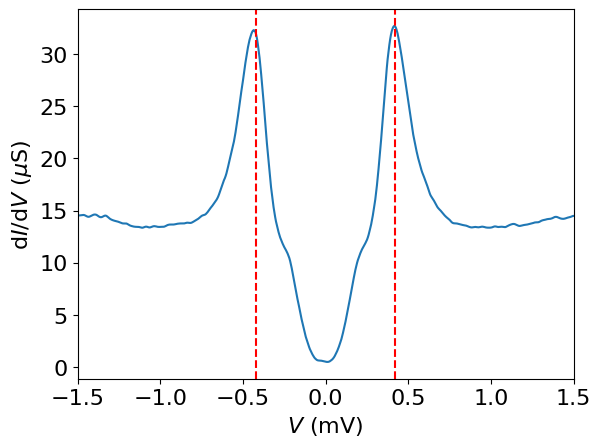
\includegraphics[width=\textwidth]{Discussion/AuNb60nm_VcExtraction.png}
         \caption{Differential conductance of AuNb device with 60 nm bridge spacing, measured at 25 mK, with the extracted $V_C$ values shown as red dashed lines.}
         \label{subfig:}
     \end{subfigure}
     \hfill
     \begin{subfigure}[t]{0.49\textwidth}
         \centering
         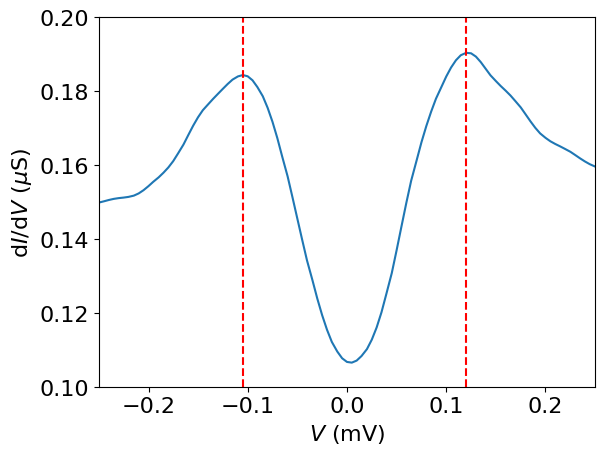
\includegraphics[width=\textwidth]{Discussion/AuNbV3DF_VcExtraction.png}
         \caption{Differential conductance of AuNb device with 50 nm niobium, measured at 30 mK, with the extracted $V_C$ values shown as red dashed lines.}
         \label{subfig:}
     \end{subfigure}
     \caption{dI/dV calculated from IV measurements, and their extracted $V_C$ values.}
     \label{fig:Vc_Extraction}
        
\end{figure}

We did this extraction for all devices for which the differential conductance shows superconducting coherence peaks. Two out of the four AuNb devices with 50 nm niobium show coherence peaks, and all four of the AuNb devices with 60 nm bridge spacing show coherence peaks. Both the AuNb devices with 50 nm niobium show critical voltages of 0.11 mV, and in the plots of the AuNb devices with 60 nm bridge spacing show critical voltages of 0.56 mV $\pm$0.16 mV . As the coherence peaks in S-I-S junctions appear at $V_C = \pm 2\Delta/e$, this allows us to estimate the average size of the induced energy gap at the tip of the leads, $\Delta_\mathrm{prox}$, to be 55 $\mu$eV and 280 $\mu$eV respectively. 

The fact that no superconducting features were observed in the IV measurements of the PdNb and AuNb indicates that either there was no induced superconducting energy gap at the tips of the leads, or that the gap was too small to be resolved. 

Only two of the four AuNb devices with 50 nm niobium showed superconductance features while all four of the four AuNb devices with 60 nm bridge spacing. This might be due to fact that the location of the tunneling gap induced through electromigration is less consistently in the center of the bridge in the AuNb devices with 50 nm niobium than in the devices with 60 nm bridge spacing. The belief that the location of the tunneling gap is less consistently at the center of the bridge for the 50 nm niobium is motivated by the fact that the center of the bridge in those devices has a double layer of gold, making the local current density and the local resistance smaller and therefore the likelihood of an electromigration induced break lower in this region, as discussed in section 5.1. In those devices where the tunnel gap forms very close to one end of the bridge, migration happens in a region where Ti and Nb are likely to be present. As discussed in the section on electromigration results, many of the devices, after they had been migrated, showed an increase in resistance when they were cooled down. This resistance increase was reversed as they were warmed back to room temperature. This type of behavior is associated with semiconductors. A possible interpretation would therefore be that when electromigration takes place far away from the center, other kinds of material such as titanium oxide for example, are mixed into the bridge material at the tunnel interface, leading to semi-conductor like behavior there. Since such a mixture has many more scattering sites than a pure metal, the diffusion would be poor which could explain the lack of observed superconductivity.  

If we compare the induced energy gaps in the devices after electromigration to the Thouless energies before electromigration, we see that the induced energy gap of the AuNb junctions with 50 nm niobium are of the same order as the determined Thouless energy of the unbroken junctions, while the induced gap in the AuNb junctions with 60 nm spacing is approximately 8 times as large as its Thouless energy before breaking. Since $L$ is halved after breaking if the break happens in the middle of the junction, and the Thouless energy scales as $1/L^2$, we expect a four-fold increase if all else stays the same. Since we see no change in the AuNb devices with 50 nm niobium thickness, and an eight-fold increase in the AuNb devices with 60 nm spacing, we can conclude that the structure of the device changes is changed during the electromigration process. The reason that the AuNb device with 50 nm niobium does not experience the four-fold increase in gap size expected based on the geometric argument may be due to the fact that the electromigration causes Ti or Nb atoms to be mixed into the Pd, which increases scattering and reduces the Thouless energy. The reason that the AuNb devices with 60 nm bridge spacing achieve an eight-fold increase might be due to the rearranging of grain boundaries, which could improve the diffusion in the gold and thereby increase the effective energy gap at the tip of the leads. In order for this effect to cause a two-fold increase in the gap, however, the mean free path would have to increase four-fold, which seems unreasonable.   

\subsection*{Andreev Reflections}

The differential conductances of three of the devices with 60 nm bridge spacing show shoulders inside the gap. 


\begin{figure}[H]
     %These plots come from numid 2 from PdNb chip 6
     \centering
     \begin{subfigure}[t]{0.49\textwidth}
         \centering
         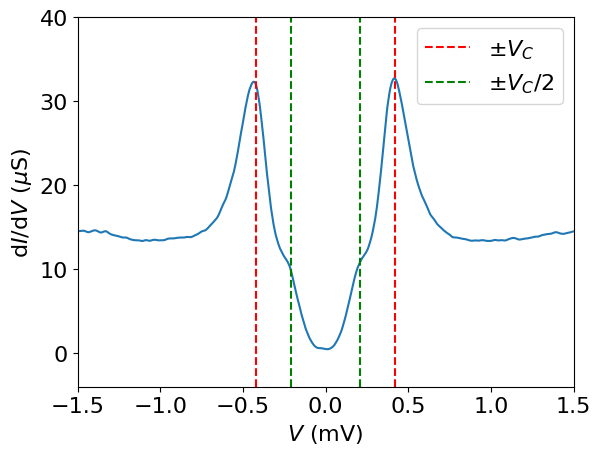
\includegraphics[width=\textwidth]{Discussion/Shoulders_106.png}
         \caption{Differential conductance of AuNb device with 60 nm bridge spacing, measured at 25 mK, with the extracted $V_C$ values shown as red dashed lines.}
         \label{subfig:}
     \end{subfigure}
     \hfill
     \begin{subfigure}[t]{0.49\textwidth}
         \centering
         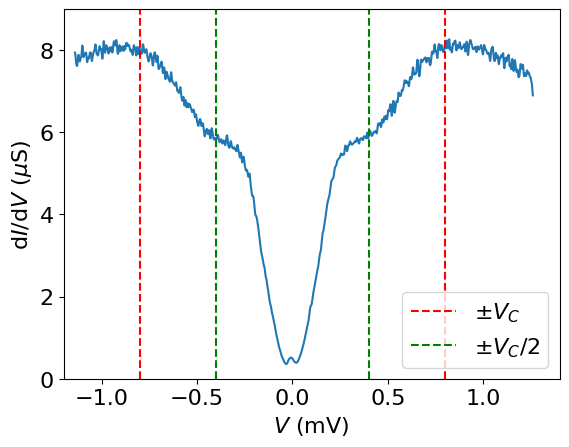
\includegraphics[width=\textwidth]{Discussion/Shoulders_70.png}
         \caption{Differential conductance of AuNb device with 50 nm niobium, measured at 30 mK, with the extracted $V_C$ values shown as red dashed lines.}
         \label{subfig:}
     \end{subfigure}
     \caption{dI/dV calculated from IV measurements, and their extracted $V_C$ values as well as the locations of the shoulders.}
     \label{fig:Shoulders_at_vc_over2}
        
\end{figure}

We attribute these shoulders to multiple Andreev reflections. When the induced energy gaps are equal on both sides of the tunnel gap, multiple Andreev reflections cause peaks in the differential conductance at $V = 2\Delta / ne$, where $n = 1,2,3,\ldots$. The size of the $n^\mathrm{th}$ peak drops off exponentially with $n$, with a decay rate dependent on the interface transparency and the phase coherence length. In the plots in figure \ref{fig:Shoulders_at_vc_over2} we can identify only the first order contribution. When the energy gaps at the tips of the leads of the SEMBJ are not equal, the locations of the Andreev reflection peaks follow a more complicated pattern, where the locations of the peaks are proportional to the energy gap at either end of the tunnel gap, or to the sum of these energy gaps. 

That the locations of the shoulders correspond to $V_C/2$ is evidence that the energy gaps are approximately equal on both sides of the tunnel gap. Since the induced energy gap is a function of the distance to the superconductor, this is evidence that the gap is forming close to the center.  

\subsection{Asymmetric Critical Current}

The results in section 4.6 show that all our devices show an asymmetric critical current upon applying a magnetic field in the perpendicular in-plane direction. This asymmetry persists across all stages of electromigrated breaking, from before any breaking has taken place until the tunnel regime. The AuNb devices with 60 nm spacing also show an asymmetry in the critical current when the magnetic field is applied in the out of plane direction. This may be attributable to the fact that the niobium layer is off-centered in those devices. That the niobium layer is off-centered means that it also somewhat resembles as an SN layer in the direction perpendicular to the current, but to a much smaller degree than in the out of plane direction. This might explain why we see this out of plane asymmetry in only those devices. 

The fact that the asymmetry of the junctions persists as the diameter of the bridge shrinks is significant, since it implies that an explanation of the asymmetry in terms of a self-field effect is less likely; since the current in those devices is very small, the strength of the generated field is correspondingly small. The characteristic magnetic field scale also remains approximately constant during the breaking process.

The consistency with which the asymmetric critical current as a function a perpendicular in-plane magnetic field is exhibited by our devices is significant since it implies that this device design can be used as a simple lithographic platform for fabricating asymmetric critical current based devices.

\subsection{Suggested Design improvements}

Based on the discussion so far, we can suggest further design changes that are likely to improve the quality of the SEMBJs. 

Since the niobium proximitizes the gold in the AuNb bilayer so strongly that the bilayer energy gap is equal to the energy gap of the bare niobium layer to within the order of one percent, we expect that the benefit increasing the thickness of the gold layer further has on the diffusion constant in the bridge will outweigh the negative effect this change has on the bilayer energy gap. Increasing the thickness of the gold would also reduce the resistivity of the bridge and make electromigration more difficult to control. However, since the results show that electromigration is highly controllable in the AuNb devices with 60 nm spacing, the level of control would remain sufficiently high even if it was reduced somewhat.

The overlap of the two gold layers in the center of the bridge in the AuNb devices with 50 nm niobium was dealt with by increasing the spacing between the two sides of the bowtie in the design. Although this removed the region of overlap, a negative side effect of this solution is that the distance from the center of the bridge to the superconductor is increased, which reduces the induced gap at the center of the bridge. An alternative solution that would not have this drawback, is to reduce the angle at which the gold layers are evaporated while keeping the bridge length the same. A potential drawback of this solution is that, since the niobium layer is placed closer to the center of the bridge, some niobium particles may be more likely to end up at the center of the bridge which might cause the contacts of the SEMBJ to be contaminated. Investigating the viability of this approach would be worthwhile.

It was mentioned in the introduction to this thesis that creating palladium based SEMBJs was of interest. As mentioned in the methods and results, it was thought that the optimizations made to the gold based SEMBJ design would also lead to improvements in the palladium based design, if palladium was resubstituted for gold. Due to time constraints, testing this hypothesis was outside the scope of this thesis, but doing so would have been an obvious next step if time had allowed for it.









